\documentclass[conference]{IEEEtran}
\IEEEoverridecommandlockouts
\pdfminorversion=7
\pdfcompresslevel=0
\pdfobjcompresslevel=0

\usepackage{cite}
\usepackage{amsmath,amssymb}
\let\proof\relax
\let\endproof\relax
\usepackage{amsthm}
\usepackage{graphicx}
\usepackage{booktabs}
\usepackage{array}
\usepackage{pifont}
\usepackage{xcolor}
\usepackage{colortbl}
\definecolor{bimrow}{HTML}{EAF2FC}
\usepackage{algorithm}
\usepackage[noend]{algpseudocode}
\usepackage{url}
\usepackage{microtype}
\usepackage[hidelinks]{hyperref}

% Preserve the reference PDF's line breaks across TeX distributions.
\hyphenation{Sec-tion bor-row-ing copy-ing de-scribe com-pu-ta-tion mech-a-nism ten-sors eval-u-ated ad-vance-ments ex-trac-tion}
% Match the reference PDF's searchable text for the large union operator.
\pdfglyphtounicode{uniontext}{22C3 FE01}

% Artifact link, set in one place: the ISPA publication branch.
\newcommand{\artifacturl}{https://github.com/assasin831/readseal-artifact/tree/ISPA}
% Framework name, set in one place (Fig. 1 and the plot legends spell it out).
\newcommand{\sys}{REALBIM}
% The two hand-placed baselines (Section V-A), named as in the plot legends: Figs. 6-7 show the standalone
% runtime ("Hand-placed"), Fig. 8 shows REALBIM with a hand-placed boundary ("REALBIM (hand-placed)").
\newcommand{\hps}{Hand-placed}
\newcommand{\hpr}{\sys{} (hand-placed)}

\newcommand{\circled}[1]{\ding{\numexpr201+#1\relax}}   % black circled digits used in Fig. 1
\newcommand{\code}[1]{\texttt{#1}}
\newcommand{\hd}[1]{\textbf{\begin{tabular}[b]{@{}l@{}}#1\end{tabular}}}   % two-line table headers
\newcommand{\op}[1]{\textsc{#1}}                          % protocol transitions (Accept, Submit, ...)
\newcommand{\MiB}{\,MiB}
\newcommand{\ms}{\,ms}
\newcommand{\Hz}{\,Hz}
\newtheorem{proposition}{Proposition}

\setlength{\textfloatsep}{10pt plus 2pt minus 2pt}
\setlength{\dbltextfloatsep}{10pt plus 2pt minus 2pt}
\setlength{\floatsep}{10pt plus 2pt minus 2pt}

% Typographic conventions: italics mark a term at its definition (and math); bold run-in heads structure
% paragraphs; small caps name protocol transitions. Frame rates are in Hz; goodput is in results/s,
% where a result is one recipient's result bundle for one frame.
% Wording conventions (r33): "late" means a missed deadline only. Where a read falls in a graph is said
% with "boundary" (a boundary near the start or the end of the graph); submission order is "first/second".

\begin{document}

\title{\sys: A Framework for Safe Early Reuse of\\ Shared GPU Buffers Across Processes}

\author{\IEEEauthorblockN{Xingbo Hui\textsuperscript{1}, Xuetao Jiang\textsuperscript{2}, Guodong Ye\textsuperscript{1}, Ruochen Shao\textsuperscript{1}, Tianyi Wang\textsuperscript{1},\\ Sicheng Wu\textsuperscript{1}, Rui Zhou\textsuperscript{1,*}, Qingguo Zhou\textsuperscript{1,*}}
\IEEEauthorblockA{\textsuperscript{1}School of Information Science and Engineering, Lanzhou University, Lanzhou, China\\
\textsuperscript{2}School of Artificial Intelligence, Zibo Polytechnic University, Zibo, China\\
\textsuperscript{*}Co-corresponding authors: zr@lzu.edu.cn, zhouqg@lzu.edu.cn}}

\maketitle

\begin{abstract}
Autonomous-driving and robotics software runs as many processes, several of which read the same large GPU tensor, such as a bird's-eye-view (BEV) feature map. Sharing that tensor instead of copying it saves memory and bandwidth, but the producer must then decide when the next frame may overwrite it. Overwriting it once submitted GPU work finishes can feed the wrong frame to a process that has not started reading, and holding it until every result is ready drops frames while the GPU idles. Our key observation is that a shared tensor has two lifetimes: its storage is needed only until the last operation that reads it, but its frame identity must last until every result is delivered. \sys{} builds on this split. Its cross-process layer, Borrow-in-Memory (BIM), protects every recipient from the moment a frame is published. Its in-process layer, ReadSeal, finds each recipient's last read by alias analysis and refuses to run if the code, model, or input layout has changed. On an A100 at 25--40\Hz, with recipients whose models stop reading the map early, releasing at the last read delivers 1.31--1.50$\times$ the timely results of holding the buffer until all results are ready, at 8--11\ms{} more mean latency. It also matches per-recipient copies without their 256\MiB{} of extra memory. \sys{} derives that point automatically. In controlled tests where one reader finished before another had submitted its reads, releasing once submitted work completed let the second reader compute on the next frame. \sys{} kept it on the correct frame and refused all 22 plans run against changed code, model state, or inputs.
\end{abstract}

\begin{IEEEkeywords}
GPU buffer reuse, zero-copy IPC, buffer lifetime, alias analysis, autonomous driving.
\end{IEEEkeywords}

% =====================================================================
\section{Introduction}
\label{sec:intro}

Autonomous-driving stacks such as Autoware run as many processes on ROS~2, the Robot Operating System~\cite{autowareonboard,ros2,ros2survey}, and several of them consume the same data (Fig.~\ref{fig:scene}). For example, a camera--LiDAR fusion node publishes a bird's-eye-view (BEV) feature map, a top-down grid of features around the vehicle. Separate processes for 3D detection, tracking, motion planning, and data recording read the map on their own schedules. We call each such process a \emph{recipient}, and each component inside a recipient that reads the map a \emph{reader}. A recipient can have several readers: BEVFusion, for instance, feeds one BEV map to both a detection and a map-segmentation head~\cite{bevfusion}.

\begin{figure}[t]
\centering
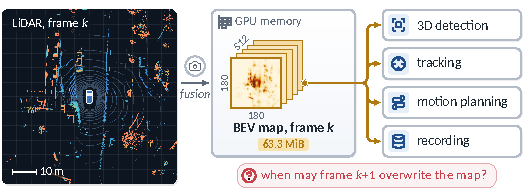
\includegraphics{figures/fig0_scene.pdf}
\caption{\textbf{One BEV map, four recipients.} Fusing each LiDAR sweep (left, from nuScenes~\cite{nuscenes}) with camera images yields a 63.3\MiB{} map in GPU memory; its front face sketches one of 512 feature channels. Sharing the map avoids four copies, but the producer must decide when frame~$k{+}1$ may overwrite it.}
\label{fig:scene}
\end{figure}

Copying the map for each recipient is expensive. Our evaluated map is a $1{\times}512{\times}180{\times}180$ fp32 tensor of 63.3\MiB~\cite{bevfusion}. Private copies for four recipients would add 256\MiB{} of device memory (64\MiB{} each after allocator rounding), and at 30\Hz{} the copying alone would read and write about 15\,GiB/s. On an automotive system-on-chip (SoC), whose GPU shares DRAM with the rest of the stack~\cite{haxconn}, that traffic is about 8\% of an AGX Orin-class module's 204.8\,GB/s~\cite{orin}, and both costs grow with every recipient. Zero-copy inter-process communication (IPC) avoids them by letting recipients map the producer's buffer~\cite{agnocast,luotcad}, and recent work and ROS~2 facilities extend this to GPU memory~\cite{hazcat,cudabackend}. The producer must then decide when it may overwrite that buffer, which we call a \emph{slot}.

Two common release policies err in opposite directions (Section~\ref{sec:motivation}). GPU work is asynchronous: a process can wait only for GPU work that has already been submitted. \emph{Stream-only release} therefore reuses the slot once all GPU work submitted so far has finished. A recipient still waiting in its queue has submitted nothing, so it later computes on the next frame, and nothing flags the mistake. A detector would then report objects seen in frame~$k{+}1$ under the timestamp of frame~$k$; at 20\Hz, a vehicle driving at 20\,m/s moves a full meter between the two. \emph{Full retention} holds the slot until every result is ready, as reference-counted zero-copy transports do when recipients keep their references until done~\cite{agnocast,ipcsharedptr}. With one slot, frames that arrive during the hold are dropped. In our 20\Hz{} trace the hold barely exceeds the frame period, so full retention drops every other frame and leaves the GPU idle in between (Fig.~\ref{fig:trace}). A second slot recovers most of these frames but costs another 64\MiB{} per shared tensor; we show that one slot, released at the right moment, delivers as many results as two (Section~\ref{sec:eval-slots}).

\begin{figure}[t]
\centering
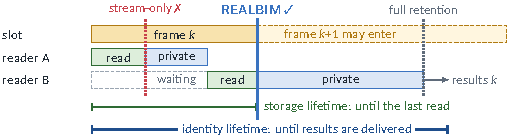
\includegraphics{figures/fig_lifetimes.pdf}
\caption{\textbf{Two lifetimes of one frame} in a recipient with readers A and B. Storage is needed until B's read, the last one; identity~$k$, until results are delivered. Stream-only release frees the slot before B reads; \sys{} frees it at the last read, so frame~$k{+}1$ can enter while B computes.}
\label{fig:lifetimes}
\end{figure}

Our key observation is that the tensor in a slot, which we call the \emph{source}, has two lifetimes (Fig.~\ref{fig:lifetimes}). Its \emph{storage lifetime} ends when the last operation that reads it completes. Its \emph{identity lifetime} lasts until every result is delivered, because those results must still name the frame they came from, much as an essay keeps citing a library book after the book has gone back to the shelf. The two can differ widely. In the TransFusion detection head that reads our BEV map, only the first of 287 operations reads the source; the rest compute on intermediate results in private memory and are unaffected when the source is overwritten. This head is not an outlier: each of the nine torchvision model tails that our analysis accepts stops reading its input within its first 12 operations (Section~\ref{sec:eval-cost}). A recipient therefore needs its \emph{borrow}, its permission to read the slot, only until its last source read completes. Full retention, copying, and early reuse then differ only in where the borrow ends: when the outputs are complete, when a private copy is complete, or at the last source read. All three must protect a recipient from the moment its frame is published, before it starts reading.

Ending the borrow at the last read is safe only if three questions can be answered. (1)~Which operation reads last? \emph{Views}, tensors that share the source's memory, extend its reads, so this \emph{read boundary} can come long after the source itself last appears. It is also easy to misplace by hand. In a ResNet-18 tail~\cite{resnet}, a residual connection reads the source again at operation~12 (Fig.~\ref{fig:boundaries}), so a boundary placed after the first read would free the source too soon. (2)~Who may still read? A reader that has not yet submitted GPU work leaves no event to wait on. (3)~Is the analyzed program the one that runs? Adding one read near our detection head's end moves its boundary from the first operation to the second-to-last (Fig.~\ref{fig:boundaries}), so a boundary derived for one model version can be wrong for the next.

We present \sys{} (REAd-Last BIM), a framework that answers these questions in two layers split at the process boundary (Fig.~\ref{fig:overview}). The producer knows only which processes receive a frame, so the cross-process layer, Borrow-in-Memory (BIM), answers question~(2). It registers a borrow for every recipient when the frame is published, before any recipient starts (Section~\ref{sec:bim}). Each recipient knows its own components, so the in-process layer, ReadSeal, answers questions~(1) and~(3). It derives each reader's boundary from its model graph and refuses a plan that no longer matches the program (Section~\ref{sec:readseal}).

With recipients whose last read comes early, on an A100 at 25--40\Hz, \sys{} delivers 1.31--1.50$\times$ the \emph{timely} results (correct and within 100\ms) of full retention at 8--11\ms{} more mean latency. It matches per-recipient copies without their memory and bandwidth cost, and it never lets a reader compute on the wrong frame, as stream-only release does. After each of 16 replayed model changes, ReadSeal rebuilds the boundary in 0.08--0.21\,s, where a hand-placed boundary is refused until a person moves it. Section~\ref{sec:discussion} discusses when a private copy is the better choice. Our contributions are:
\begin{itemize}
\item \textbf{Two lifetimes for shared GPU tensors}, which make full retention, copying, and early reuse one mechanism that ends a borrow at different points.
\item \textbf{BIM: protection from publication} (Section~\ref{sec:bim}), which covers recipients that have not yet submitted any GPU work, as no event-based policy can, and ends each borrow at a GPU completion event.
\item \textbf{ReadSeal: a derived, checked release point} (Section~\ref{sec:readseal}), which finds each reader's last read by alias analysis and refuses a plan whose code, model, or input layout has changed.
\end{itemize}

% =====================================================================
\section{Background and Motivation}
\label{sec:motivation}

\begin{figure*}[t]
\centering
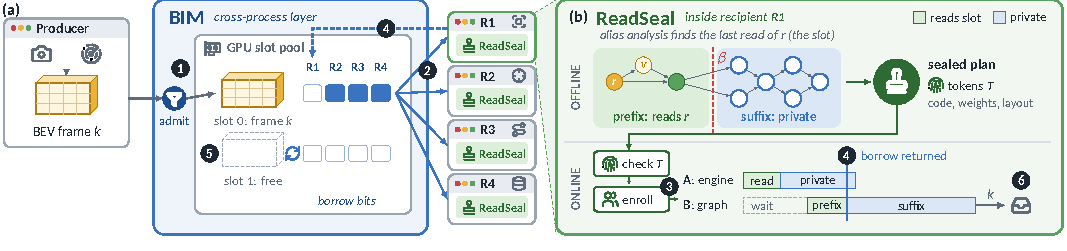
\includegraphics{figures/fig1_framework.pdf}
\caption{\textbf{\sys's two layers.} (a)~BIM, in the producer and shared memory, keeps a pool of GPU slots with one borrow bit per recipient and slot. (b)~ReadSeal, inside each recipient: offline, alias analysis splits a reader's graph at its last read~$\beta$ of source~$r$ into a prefix that reads~$r$ and a private suffix, and tokens~$T$ bind the plan to code, weights, and input layout; online, the recipient checks~$T$ (also at each stage entry) and enrolls readers A, a TensorRT engine, and B, an exported graph. Numbers follow frame~$k$ (Section~\ref{sec:bim}).}
\label{fig:overview}
\end{figure*}

\begin{figure}[t]
\centering
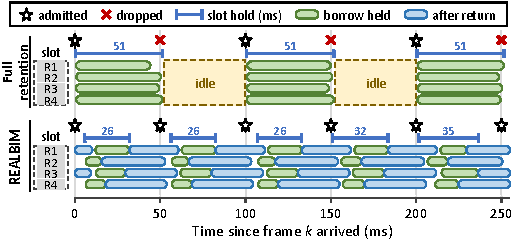
\includegraphics{figures/fig2_trace.pdf}
\caption{\textbf{Full retention refuses frames while the GPU idles.} Measured one-slot trace at 20\Hz; R1--R4 are the recipients, and labels give slot hold times in ms. Full retention's 51\ms{} hold just exceeds the 50\ms{} period, so every other frame is refused. Under \sys, each recipient's work after its borrow return overlaps the next frame.}
\label{fig:trace}
\end{figure}

\begin{figure}[t]
\centering
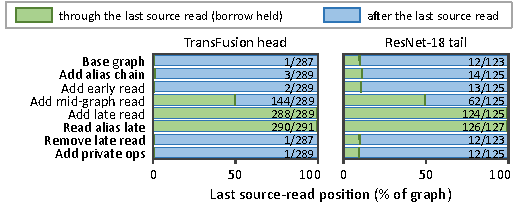
\includegraphics{figures/fig3_boundaries.pdf}
\caption{\textbf{Model edits move the last source read.} Each bar is a graph snapshot that applies one edit to the base graph (Remove late read undoes Add late read). Green marks the operations up to the last source read, during which the recipient holds its borrow; labels give that operation's index\,/\,total operations.}
\label{fig:boundaries}
\end{figure}

This section gives the GPU background and shows where existing policies end the borrow (Table~\ref{tab:options}).

\textbf{GPU background.} A \emph{kernel} is a function executed on the GPU. A process places kernels in a \emph{stream}, a queue that the GPU runs in order, and continues without waiting; a read ends when its kernel completes. An \emph{event} marks a position in a stream and completes after the preceding work. PyTorch's caching allocator reuses freed memory in stream order~\cite{pytorch}, and \code{record\_stream} extends this to other streams by waiting for work already enqueued on them~\cite{recordstream}. CUDA IPC lets another process map a device buffer and wait on shared events, but an event marks only work already enqueued: no process can wait on reads another has not submitted.

\textbf{Stream-only release.} A policy that waits only for submitted work, such as \code{record\_stream} or a read event, releases the slot once the other recipients' reads complete, although a recipient still waiting in its queue has enqueued nothing. The same gap opens inside one recipient whose readers run on different runtimes, as when BEVFusion's detection and segmentation heads read one map~\cite{bevfusion} and one of them is compiled to an inference engine. Our running example (Fig.~\ref{fig:overview}b) models this with two readers. Engine~A, built with NVIDIA's TensorRT, stands in for the compiled head: it runs a convolution, ReLU, and pooling stage on the map and signals an input-consumed event once it has read its input~\cite{tensorrt}. Graph~B is the detection head, exported from PyTorch, and receives the map as a view through an adapter that does not read it. So when A's event completes, B has submitted nothing and there is no event to wait on: stream-only release makes the slot reusable while B still needs it (Section~\ref{sec:eval-safety} tests this ordering). ROS~2's CUDA buffer backend offers both choices: destroying a read handle after the engine's read gives stream-only release; holding it, full retention~\cite{cudabackend}.

\textbf{Copying the source.} A private copy lets a recipient compute after the slot is reused, but the copy itself reads the source, so the slot must stay protected until the copy completes. Our \emph{clone-on-accept} baseline copies the source at acceptance, relies on BIM until then, and ends each borrow when the copy completes.

\begin{table}[t]
\caption{Release policies for four recipients. Extra memory counts input copies beyond the shared slot.}
\label{tab:options}
\centering
\footnotesize
\setlength{\tabcolsep}{2.2pt}
\begin{tabular}{@{}lllll@{}}
\toprule
\hd{Policy} & \hd{Extra\\memory} & \hd{Slot reusable\\after} & \hd{Read\\boundary} & \hd{Wrong\\frame?} \\
\midrule
Stream-only              & ---       & submitted reads & ---      & possible \\
Full retention           & ---       & all outputs     & ---      & no \\
Clone-on-accept          & 256\,MiB  & all copies      & the copy & no \\
Hand-placed              & ---       & all last reads  & by hand  & no \\
\rowcolor{bimrow}
\sys                  & ---       & all last reads  & derived  & no \\
\bottomrule
\end{tabular}
\end{table}

% =====================================================================
\section{The \sys{} Framework and Its BIM Layer}
\label{sec:bim}

\sys{} tracks the two lifetimes separately (Fig.~\ref{fig:overview}). A frame identity, attached when the frame is written and carried by every result, covers the identity lifetime; per-recipient borrows cover the storage lifetime. BIM lives in the producer, which owns a pool of $N$ reusable GPU slots on one machine, and in shared memory; ReadSeal (Section~\ref{sec:readseal}) runs inside each recipient and decides when its borrow ends. The layers meet at one borrow bit per recipient and slot, which BIM sets before the recipient can read and ReadSeal clears after its last source read. One borrow covers all of a recipient's readers, even those yet to submit work. A recipient \emph{returns} its borrow by clearing its bit; the slot becomes reusable when its last bit clears.

\textbf{Life of a frame.} The numbers in Fig.~\ref{fig:overview} follow frame~$k$. BIM's producer \emph{admits} it into a free slot (\circled{1}), \emph{commits} it by setting every recipient's borrow bit, and then sends each recipient a small descriptor (\circled{2}). The descriptor carries the frame identity (producer instance and sequence number), a storage locator, and the layout to read. In each recipient, ReadSeal \emph{accepts} the request, checks its plan, and \emph{enrolls} the readers (\circled{3}); after the last source read, the recipient returns its borrow (\circled{4}). A slot whose bits are all clear takes the next frame (\circled{5}), while results labeled~$k$ are still being delivered (\circled{6}). Descriptors travel over a control plane such as ROS~2, recipients map the tensor through PyTorch's CUDA IPC support~\cite{pytorch}, and BIM rejects stale identities and incompatible layouts.

\textbf{Borrow bits and admission.} A process-shared lock protects slot reservation, the frame sequence, and one borrow bit per recipient, set while that recipient may still read the slot. An arriving frame takes a slot whose bits are all clear; if none is free, the producer drops the frame instead of waiting. Once the frame is written, the producer commits it by setting every recipient's bit before sending any descriptor. A recipient still waiting in its queue is therefore protected, because its bit was set before it could possibly read. Clearing the last bit makes the slot reusable without deallocating or unmapping it. If frame~$k$ is committed at time~$c_k$ and recipient~$j$ returns its borrow at time~$t_{j,k}$, the slot is held for $H_k$. With one slot, a frame arriving at time~$a$ is admitted only if
\begin{equation}
a\;\ge\; c_k+H_k, \qquad H_k=\max_j t_{j,k}-c_k. \label{eq:hold}
\end{equation}
Under full retention, $t_{j,k}$ is when $j$'s outputs complete; under \sys, it is when $j$'s last source read completes (Section~\ref{sec:enroll}), and the shorter hold admits more of the arriving frames. Each admitted frame gives every recipient one \emph{request}, which the recipient accepts when it takes the request from its queue. The request stays outstanding until its result reaches the output sink. An optional admission cap~$K$ bounds the pipeline's outstanding requests; a frame is admitted only if a slot is free and the cap allows it.

% =====================================================================
\section{The ReadSeal Layer: Checked Borrowing}
\label{sec:readseal}

ReadSeal prepares a \emph{plan} once per model version and checks it each time a recipient processes a frame (Algorithm~\ref{alg:readseal}). The plan records where the graph stops reading shared storage, which components may read it, and which program version was analyzed. One execution of a plan is an \emph{invocation}.

\subsection{Deriving the Read Boundary}
\label{sec:derive}

\begin{algorithm}[t]
\caption{\sys{} per frame: BIM's publication and ReadSeal's plan and invocation. $b_{s,j}$: borrow bit of recipient $j$ on slot $s$; $U_j$: readers of $j$; $T$: binding tokens.}
\label{alg:readseal}
\footnotesize
\begin{algorithmic}[1]
\Procedure{Publish}{frame $k$}\Comment{producer (BIM)}
\State \textbf{if} no slot is free or cap $K$ has no room for $k$, \textbf{drop} $k$
\State write $k$ into a free slot $s$; \emph{commit}: set $b_{s,j}$ for all $j$
\State send each recipient a descriptor of $(k,s)$
\EndProcedure
\Procedure{BuildPlan}{graph $G$}\Comment{offline, per model version}
\State $Q_r$ by \eqref{eq:reads}, $\beta$ by \eqref{eq:boundary}; split $G$ at $\beta$; record $U_j$, $T$
\EndProcedure
\Procedure{Invoke}{plan, frame $k$}\Comment{recipient $j$}
\State check $T$; keep identity $k$ for every output
\State enroll every reader in $U_j$ before any of them submits GPU work
\State submit the stages in declared order, checking $T$ at each entry
\State \textbf{on} failed check: cancel unsubmitted reads, drain, publish nothing
\State \textbf{on} each completed or cancelled read: \textbf{if} \eqref{eq:return} holds, clear $b_{s,j}$
\State \textbf{on} completed outputs: publish them with identity $k$
\EndProcedure
\end{algorithmic}
\end{algorithm}

The analysis runs on each reader's exported graph~\cite{pytorch2}: a directed acyclic graph (DAG) of operations with fixed tensor shapes. Only the storage lifetime needs analysis, because every result carries the frame identity attached at acceptance. Sharing propagates through views: a slice of the source is a view, so an operation on the slice still reads the source, whereas a convolution reads the source but writes fresh storage, so operations on its output do not.

Formally, let $S(v)$ be the set of shared roots whose storage a value~$v$ may alias, with $S(r)=\{r\}$ for the source~$r$. For an operation~$o$ with inputs $v_i$ and output $v_o$, let $\mathcal{A}_o$ index the inputs the output may alias and $\mathcal{R}_o$ the inputs $o$ reads. Then
\begin{equation}
\begin{aligned}
S(v_o)&=\textstyle\bigcup_{i\in \mathcal{A}_o} S(v_i),\\
Q_r&=\{\, o : \exists\, i\in \mathcal{R}_o,\; r\in S(v_i) \,\},
\end{aligned}\label{eq:reads}
\end{equation}
where $Q_r$ is the set of operations that may read the source. With the operations numbered $o_1,\dots,o_n$ in execution order, the read boundary is the position of the last one in $Q_r$,
\begin{equation}
\beta=\max\{\, i : o_i\in Q_r \,\}, \label{eq:boundary}
\end{equation}
and the \emph{prefix} $o_1,\dots,o_\beta$ contains every source read, while the \emph{suffix} $o_{\beta+1},\dots,o_n$ computes the remaining results in private storage. If no operation reads the source, $Q_r$ is empty and we set $\beta=0$. Fig.~\ref{fig:boundaries} labels each snapshot with $\beta/n$; the base head has $\beta=1$ and $n=287$.

The sets $\mathcal{A}_o$ and $\mathcal{R}_o$ come from reviewed summaries of 42 operator variants in ATen (PyTorch's operator library), plus fixed-index tuple selection. Each summary conservatively counts every input as read and lets an output share storage whenever the operator's declared signature permits it. Plan construction rejects what it cannot analyze: unsupported in-place updates, calls into code it cannot inspect, and source views that leave the graph. The implementation compiles the prefix and suffix into separate executable stages, and a CUDA event after the prefix marks the end of its source reads.

\subsection{Enrolling Readers Before Submission}
\label{sec:enroll}

BIM already protects each recipient from commit on. When the recipient accepts its request, ReadSeal \emph{enrolls} (registers) all of its readers before any of them submits GPU work. Each reader~$u$ marks its last source read with a completion event: A's input-consumed event or the event after B's prefix. Let $U_j$ be the readers of recipient~$j$. Then $j$ returns its borrow for frame~$k$ at the first moment when
\begin{equation}
\forall u\in U_j:\quad \mathit{done}_u \lor \mathit{cancelled}_u, \label{eq:return}
\end{equation}
where the predicate $\mathit{done}_u$ becomes true when $u$'s completion event completes, and $\mathit{cancelled}_u$ when $u$ is cancelled before submission. Every enrolled reader takes part in this condition, even one that has enqueued nothing: when A's event completes, B's read is still pending, so the bit stays set. Once all recipients have returned their borrows, the producer can write the next frame while $j$'s suffix keeps computing results labeled~$k$.

% Fig. 6 (fig5_delivery) is defined here so that it floats to the top of the page where Section V starts.
% ---------------------------------------------------------------------
\begin{figure*}[t]
\centering
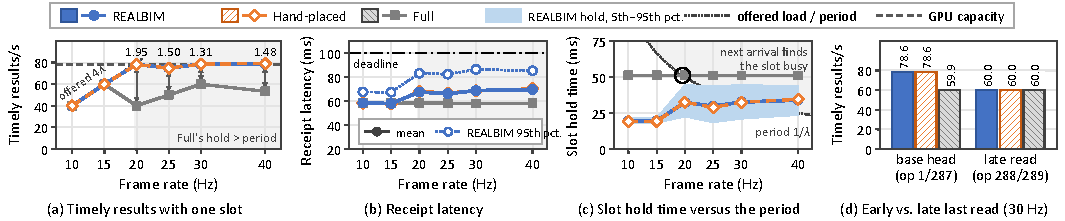
\includegraphics{figures/fig5_delivery.pdf}
\caption{\textbf{Early reuse raises one-slot delivery under load, at a latency cost.} One slot, no pipeline-wide cap~$K$, six runs per condition and policy; each frame offers four recipient results. Hand-placed releases at the same point as \sys{} by design (Section~\ref{sec:eval}). (a)~Labels give \sys/Full ratios. (b)~Mean receipt latency and \sys's mean per-run 95th percentile. (c)~Mean hold and \sys's 5th--95th percentile; shading marks where Full's hold exceeds the frame period. (d)~Moving the last read to the graph's end removes the gain.}
\label{fig:delivery}
\end{figure*}

\subsection{Binding Plans to Execution}
\label{sec:bind}

After a model update, a patched function or global variable, or an input with different strides, a plan's boundary can fall before a read that the running program performs. The producer would then overwrite the source while it is still in use. At construction, ReadSeal captures the functions to run and copies the model's weights and other state into plan-owned storage, so later edits by the caller cannot change a plan in use; the hand-placed baselines keep the same copy.

ReadSeal then records \emph{binding tokens}~$T$ for everything the boundary depends on. Code and global variables define the operations. Model storage and version tell whether the model the caller is about to run is still the one the plan was built from. The input layout matters because aliasing depends on strides: a reshape returns a view only when the strides allow it. The compiled stages are what actually executes. At acceptance and at each stage entry ReadSeal compares $T$ with the values $\hat T$ for the execution about to run and proceeds only if $\hat T=T$. A failed check cancels unsubmitted reads, drains started work, and publishes nothing. Applications supply the exported graph, each engine's last-input-read event, and component and output dependencies; new operators need reviewed summaries.

\subsection{Correctness Conditions}
\label{sec:correctness}

The analysis must include every operation that can read the source. It assumes that operator summaries conservatively describe reads and storage sharing, kernels obey those summaries, and the graph executes in the analyzed order.

\begin{proposition}
Under these assumptions, $Q_r$ in Eq.~\eqref{eq:reads} contains every operation that can read the source, so no operation after~$o_\beta$ reads it.
\end{proposition}
\begin{proof}[Proof sketch]
By induction over graph order, the union in Eq.~\eqref{eq:reads} keeps $r$ in $S(v)$ for every value~$v$ that may alias the source, and the read rule places each operation consuming such a value in~$Q_r$.
\end{proof}

The runtime further requires that each reader's completion event follow its source reads, that mappings stay valid, and that identities stay unique while referenced. Under these conditions, enrolling readers before submission (Algorithm~\ref{alg:readseal}), returning a borrow only when Eq.~\eqref{eq:return} holds, and overwriting only after all bits clear preserve the source until every reader finishes, while results keep the identity captured at acceptance.

% =====================================================================
\section{Evaluation}
\label{sec:eval}

% Fig. 7 (fig6_slots) is defined at the start of Section V so that it floats to the page after Fig. 6.
\begin{figure*}[t]
\centering
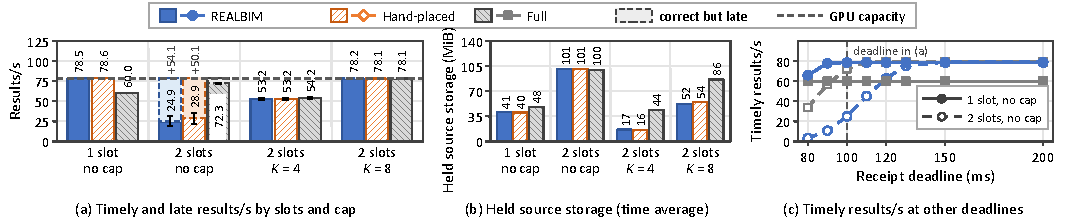
\includegraphics{figures/fig6_slots.pdf}
\caption{\textbf{One \sys{} slot matches full retention with two slots and an admission cap} (30\Hz; six runs per condition and policy). $K$ caps outstanding recipient requests. (a)~Solid: timely results; dashed: correct but late; whiskers: 95\% intervals. (b)~Time-averaged source storage held by unreturned borrows. (c)~The same runs re-scored at other deadlines.}
\label{fig:slots}
\end{figure*}

We ask what releasing at the last read gains and costs (Sections~\ref{sec:eval-delivery}--\ref{sec:eval-mixed}), whether \sys{} keeps every reader on its frame as reads are reordered and models change (Section~\ref{sec:eval-safety}), and what its checks cost (Section~\ref{sec:eval-cost}). The hand-placed baselines release at the same point as \sys{} and so match its delivery by design: the throughput gain comes from where the borrow ends. Deriving that point pays off in safety, which Section~\ref{sec:eval-safety} measures, including a residual read that a boundary placed by hand after the first read would miss.

\subsection{Setup}
\label{sec:eval-setup}

\textbf{Platform.} We evaluate cross-process reuse on one NVIDIA A100 PCIe 40\,GB GPU. The producer, four recipients, and an output sink are separate processes that communicate through multiprocessing queues and share storage and events through CUDA IPC. To isolate reuse and admission from feature extraction, the producer replays saved BEV features. The runtime uses PyTorch 2.1.2, CUDA 12.1, and TensorRT 10.3. Without NVIDIA's Multi-Process Service (MPS), recipient kernels take turns on the GPU rather than running concurrently~\cite{bakita24}. Records, validators, and analysis scripts are public.\footnote{\url{\artifacturl}.}

\textbf{Workload.} Graph~B is BEVFusion's functional TransFusion head~\cite{bevfusion,transfusion}, exported with 287 operations, and engine~A, the stand-in for a compiled second head, runs the head's shared convolution, ReLU, and global average pooling in TensorRT (Section~\ref{sec:motivation}). The producer publishes precomputed 63.3\MiB{} feature maps from three fixed nuScenes-mini frames~\cite{nuscenes}. Four recipients run identical compositions in the sweeps; Section~\ref{sec:eval-mixed} varies their components. The correctness, model-change, and cost tests use a ResNet-18 tail~\cite{resnet}: its residual stages and classifier read saved first-layer activations.

\textbf{Policies.} All policies share the pool, workloads, queues, and admission settings. \emph{\sys} uses both layers, \emph{Full} is full retention, and \emph{Clone-on-accept} gives each recipient a private input copy when it accepts a request. \emph{\hps} is a separate runtime that enrolls both readers, releases at a boundary set by hand, and checks code and model digests; it tests early reuse independently of our code (Sections~\ref{sec:eval-delivery} and~\ref{sec:eval-slots}). \emph{\hpr} is \sys{} with its boundary set by hand instead of derived, so the two differ only in where the boundary comes from (Section~\ref{sec:eval-mixed}).

\textbf{Metrics.} The producer schedules frames at rate~$\lambda$, in Hz. Each frame should yield four \emph{results}, one output bundle per recipient, so the offered load is $4\lambda$ results/s. A result is \emph{timely} if it passes source-identity and reference-output checks and reaches the output sink within 100\ms{} of the frame's planned arrival, including device-to-host transfer and IPC; Fig.~\ref{fig:slots}c re-scores the slot runs at other deadlines. \emph{Receipt latency} runs from planned arrival to sink receipt, and \emph{slot hold time} from commit to the last borrow return. Section~\ref{sec:eval-mixed} uses the \emph{complete-frame timely fraction}: the share of scheduled frames, refused ones included, with all four results timely.

\textbf{Runs and statistics.} Table~\ref{tab:runs} lists the experiments. The producer drops frames rather than blocking, so every policy sees the same offered load. In the sweeps, each recipient holds at most two \emph{pending} requests (queued, not yet accepted) and four \emph{in flight} (accepted, results not yet delivered). A run has 2\,s of warm-up, 12\,s of measured arrivals, and a complete drain, in randomized order. Because these runs report ratios and paired differences, brackets give pointwise 95\% intervals from 20,000 paired whole-run bootstrap draws. The campaigns report per-policy fractions with pointwise 95\% $t$ intervals; they use queues of eight, 10\,s of warm-up, and 30\,s of measurement.

\begin{table}[t]
\caption{Experiments. Runs are per policy and condition; $K$ is the admission cap.}
\label{tab:runs}
\centering
\scriptsize
\setlength{\tabcolsep}{2.4pt}
\begin{tabular}{@{}lllllll@{}}
\toprule
\hd{Experiment} & \hd{Policies} & \hd{Rate\\(Hz)} & \hd{Slots,\\$K$} & \hd{Runs} & \hd{Metric} & \hd{Where} \\
\midrule
Rate sweep  & R H F      & 10--40 & 1, off        & 6          & results/s, ms   & Fig.~\ref{fig:delivery}a--c \\
Late read   & R H F      & 30     & 1, off        & 6          & results/s       & Fig.~\ref{fig:delivery}d \\
Slot study  & R H F      & 30     & 1--2, off/4/8 & 6          & results/s, MiB  & Fig.~\ref{fig:slots} \\
Campaigns   & R Rh F C   & 30     & 1, off        & 6 (+12)    & \% frames, p99  & Fig.~\ref{fig:mixed} \\
Vs.\ copies & R C        & 20--40 & 1, off        & 168        & results/s, p99  & \S\ref{sec:eval-mixed} \\
Safety      & R H Rh S   & ---    & ---           & 6/96/22/16 & identity, outputs & \S\ref{sec:eval-safety} \\
Cost        & R H        & ---    & ---           & 8$\times$50 & ms per call    & \S\ref{sec:eval-cost} \\
\bottomrule
\multicolumn{7}{@{}p{\linewidth}@{}}{Policies: R \sys, H \hps, Rh \hpr, F Full, C Clone-on-accept, S stream-only.}
\end{tabular}
\end{table}

\subsection{Early Reuse Raises Delivery Under Load}
\label{sec:eval-delivery}

Early reuse pays off once the frame period drops below Full's hold time (Fig.~\ref{fig:delivery}a). Because the recipients take turns on the GPU and Full's 51\ms{} hold spans nearly all of their computation, the GPU can finish at most about four results per 51\ms, or 78 results/s (dashed line). From 20\Hz{} on, the offered load reaches this capacity, so each frame Full refuses leaves GPU time unused. At 20\Hz, where Full accepts only every other frame, \sys{} delivers 1.95$\times$ Full's timely results, and at 25--40\Hz{} 1.31--1.50$\times$ as many, near capacity. \sys{} stays within 0.2 results/s of \hps{} throughout.

The gain comes from a shorter hold: Full holds the slot for about 51\ms, whereas \sys{} returns it once the last recipient's first operation has run, in 30--34\ms, since the recipients take turns on the GPU (Fig.~\ref{fig:delivery}c). The shorter hold lets the next frame enter while private computation continues, which fills the idle gaps of Fig.~\ref{fig:trace}. The dip at 25\Hz{} comes from periodic arrivals. The 40\ms{} period is shorter than \sys's longer holds (95th percentile 44\ms), so after each refusal the slot waits a full period for the next arrival, which comes sooner at 30 and 40\Hz.

The extra admitted work queues on the GPU, which costs latency. At 20--40\Hz, \sys's mean latency is 8--11\ms{} higher than Full's and its per-run 95th percentile 15--19\ms{} higher (Fig.~\ref{fig:delivery}b). At 30\Hz{} \sys's delivery lead holds for deadlines from 100 to 200\ms{} and narrows at 80\ms, where more of this queued work arrives late (Fig.~\ref{fig:slots}c).

\label{sec:eval-late}The gain depends on where the last read falls. Adding a read at operation 288 of 289 (Fig.~\ref{fig:boundaries}, Add late read) leaves almost nothing to overlap: \sys's hold reaches Full's, and all three policies deliver 60.0 results/s at 30\Hz{} (Fig.~\ref{fig:delivery}d).

\subsection{One Slot Matches Two, and Two Need a Cap}
\label{sec:eval-slots}

A second slot is the usual remedy for Full's refusals (Fig.~\ref{fig:slots}a). At 30\Hz, two-slot Full with $K{=}8$ delivers 78.1 results/s, and one-slot \sys{} delivers 78.5, one 64\MiB{} buffer fewer per shared tensor. The second slot also makes the cap decisive: $K{=}4$ holds every policy to 53--54 results/s, and without a cap work arrives late.

With one slot, the hold time in Eq.~\eqref{eq:hold} paces \sys's admissions. A second slot removes that pacing and lets requests queue before the GPU can start them. As with bufferbloat in networks, the longer queue adds delay without adding throughput: without a cap, two-slot \sys{} delivers only 24.9 timely results/s, and another 54.1 arrive correct but late. Full's longer hold still throttles its arrivals, so it delivers 72.3. \hps{} behaves like \sys, and looser deadlines recover both (Fig.~\ref{fig:slots}c).

At $K{=}8$, all three policies reach similar delivery (Fig.~\ref{fig:slots}a), but \sys{} returns borrows sooner. The source storage held by borrows therefore averages 52.3\MiB{} under \sys{} against 86.4\MiB{} under Full (Fig.~\ref{fig:slots}b), memory that an allocator could lend to other work.

\subsection{Jitter, Mixed Recipients, and Copying}
\label{sec:eval-mixed}

\begin{figure}[t]
\centering
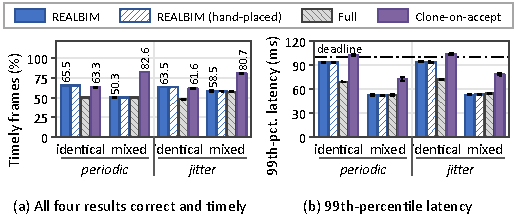
\includegraphics{figures/fig7_mixed.pdf}
\caption{\textbf{Complete-frame delivery and tail latency with jitter and mixed recipients} (30\Hz, one slot, no pipeline-wide cap; six runs per bar; whiskers: 95\% $t$ intervals). (a)~Share of the 900 scheduled frames per run whose four results are all correct and timely. (b)~Per-run 99th-percentile latency of frames whose four results are all correct. \emph{Identical}: four copies of the composition; \emph{mixed}: four component profiles, one with its last read at the graph's end.}
\label{fig:mixed}
\end{figure}

In the campaigns (Fig.~\ref{fig:mixed}), arrivals are periodic or displaced by up to 0.8 of a period (\emph{jitter}), and recipients are either \emph{identical} copies of the composition or \emph{mixed}: the native engine alone, the exported head alone, their composition, and a composition whose last read is at the graph's end.

With identical recipients, \sys{} completes 65.5\% of frames on time under periodic arrivals, i.e., 78.6 of the 120 results/s offered, the GPU's capacity (Section~\ref{sec:eval-delivery}), and 63.5\% with jitter, about 15.5 percentage points above Full in both cases. With mixed recipients, the recipient that reads at the end holds the slot for all four, and \sys{} stays less than one point above Full (Fig.~\ref{fig:mixed}a). Jitter raises mixed-recipient delivery from 50.3\% to 58.5\% for \sys{} and from 50.0\% to 57.5\% for Full, as irregular gaps let more frames past that recipient's hold. Across both campaigns, including 12 runs in which every recipient reads at the end, \hpr{} stays within 0.13 percentage points of \sys.

Clone-on-accept returns its borrow when the copy completes, however long computation then reads the private copy. With identical recipients it completes about two points fewer frames on time than \sys. With mixed recipients it completes 22--32 points more, because no computation holds the slot, at a 256\MiB{} higher sampled device peak and 20--25\ms{} more 99th-percentile latency.

The 168-run comparison agrees. With early last reads, \sys{} delivers 0.4--0.9 results/s more than Clone-on-accept at 20, 30, and 40\Hz, and 2.75 [2.47, 3.03] fewer at its 25\Hz{} dip. With every last read at the end, at 30\Hz, Clone-on-accept delivers 76.4 results/s to \sys's 60.0 (paired gain 16.39 [16.06, 16.72]). It also raises mean per-run 99th-percentile latency from 68.7 to 101.1\ms{} and device peak by 256\MiB.

\subsection{Safety Across Reordering and Model Changes}
\label{sec:eval-safety}

We first reorder reads on purpose. In six controlled tests, engine~A's input-consumed event completes before graph~B submits its reads. Under stream-only release, B's outputs matched the replacement frame in every test, because recording stream use cannot cover reads that have not been submitted~\cite{recordstream}; under \sys{} and \hps, they matched the admitted frame. Under load, all 109,592 results delivered by \sys, \hps, and Full in the 144 rate and late-read runs carried their admitted identity and matched reference outputs.

We then change the models. In 96 ordered-overwrite cases (eight graph snapshots per model, three inputs, and two methods), the source was overwritten as soon as the regenerated boundary had completed, and the outputs matched the unsplit model's exactly. They include the ResNet-18 tail, whose derived boundary sits at the residual read at operation~12 (Fig.~\ref{fig:boundaries}, right). A boundary placed by hand after the first read would have freed the source under that read, unnoticed. Binding checks rejected all 22 attempted substitutions of plan, code, globals, model state, or input before the affected stage ran.

Finally, we replay 16 controlled transitions: the 14 graph edits of Fig.~\ref{fig:boundaries}, one folding of batch normalization into the preceding convolution, and a public ResNet-18 to ResNet-50 substitution, whose binding check runs on the CPU. Some move the last source read; others only renumber it or leave it in place. Binding checks reject every outdated hand-placed plan, which then waits for a person to move its boundary. ReadSeal rebuilds every updated plan in 0.08--0.21\,s on the CPU, with no annotations. In the mixed-recipient campaign, adding a read at the end made the old boundary of \hpr{} fail its binding check until the boundary was moved; all 24 update cases then gave exact outputs.

\subsection{Execution Cost and Coverage}
\label{sec:eval-cost}

An isolated-process test times recipient acceptance to output dispatch (8 process repetitions of 50 randomized invocations per method; three inputs; both models with and without a read added at the end). ReadSeal's checks add 0.8--0.9\ms{} per invocation, mostly at acceptance and stage submission: 8\% over \hps{} for the base head (11.8\ms{} against 10.9\ms) and 22--23\% for the lighter ResNet tail. In the pipelines above this cost overlaps GPU work; even at 10 and 15\Hz, \sys's mean receipt latency is within 0.4\ms{} of \hps's. A static survey of the tails of 14 torchvision models accepts nine, with boundaries in their first 1--12 operations, and rejects five for unsupported operators.

% =====================================================================
\section{Discussion}
\label{sec:discussion}

\textbf{Borrow or copy.} Where the last read falls decides between borrowing and copying. With early last reads, a borrow ends about when a copy would, so borrowing delivers as much without the copies' memory and bandwidth. When a reader's last read comes at the end of its graph, copying delivers more (Fig.~\ref{fig:delivery}d; Section~\ref{sec:eval-mixed}). Because \sys{} derives every boundary before the reader runs, the choice can follow from the plan rather than from measurement.

\textbf{Beyond the A100.} The delivery gain depends on how the hold compares with the frame period (Eq.~\eqref{eq:hold}), not on memory capacity. A shared-DRAM SoC changes the price of the alternatives. There, a second slot or a private copy takes memory and bandwidth from the rest of the stack~\cite{haxconn}; on our 40\,GB card, a 64\MiB{} slot is small beside a 5\,GiB device peak. We therefore expect borrowing to save more on an SoC.

\textbf{Limitations.} Our measurements come from one A100 without MPS, where recipients take turns on the GPU~\cite{reef,orion}, and from replayed features rather than a ROS~2 stack with its BEV front end. Our fixed slot pool does not yet lend the storage that early returns free, so device peak is the same for every policy (5,078\MiB{} with one slot, 5,142\MiB{} with two). The six ordered tests show that stream-only release can compute on the wrong frame, not how often. The prototype runs declared topologies with single-stream stages. A slow recipient holds the slot for everyone (Section~\ref{sec:eval-mixed}), and a crashed one until recovery stops its GPU work.

% =====================================================================
\section{Related Work}
\label{sec:related}

\textbf{Zero-copy IPC and cross-process lifetime.} Shared-memory transports let ROS~2 subscribers read publisher-owned messages in place~\cite{agnocast,luotcad}. Hazcat and ROS~2's \code{rosidl::Buffer} backends carry zero-copy into device memory~\cite{hazcat,cudabackend}, and NvSciStream lets each consumer return a buffer on its own but leaves where to return it to the application~\cite{nvscistream}. Agnocast keeps a message until every subscriber has dropped its reference, tracked by \code{ipc\_shared\_ptr} with one bit per subscriber~\cite{ipcsharedptr}. BIM uses the same kind of per-recipient bits, but GPU completion events, not reference drops, clear them, and results carry frame identities. That change lets ReadSeal end a borrow at a derived, checked last read.

\textbf{Timing and GPU sharing.} Real-time analyses of ROS~2 bound chain latency, data age, and the time disparity of fused messages~\cite{ros2survey}, assuming that each message keeps its data and timestamp until consumed, which \sys{} guarantees for shared GPU tensors. Multi-tenant GPU systems preempt or interleave co-located models~\cite{reef,orion} or schedule around SoC memory contention~\cite{haxconn}, but manage memory that one runtime allocates, not tensors shared across processes.

\textbf{Last use and reclamation.} Memory planners and borrow checkers track lifetimes, also over GPU memory, but see every use in one program~\cite{telamalloc,descend}; a producer sees neither its recipients' programs nor their unsubmitted reads. Read-copy-update (RCU)~\cite{rcu} reuses memory once no reader can hold it but protects only readers that have announced themselves. BIM's commit (Section~\ref{sec:bim}) instead opens every recipient's read-side section, the interval in which it may read, on its behalf, and ReadSeal closes it at the last read. ReadSeal's bindings, like PyTorch~2's guards~\cite{pytorch2}, reject execution whose assumptions changed, but where a failed guard recompiles, a failed binding refuses to run, because another process relies on the boundary.

% =====================================================================
\section{Conclusion}

Sharing one GPU buffer among processes saves the memory and bandwidth of private copies, but only if the producer knows when it may overwrite it. The answer lies in separating two lifetimes: storage is needed until the last read, often a model's first operation, while identity must last until every result is delivered. Full retention, copying, and early reuse then differ only in where the borrow ends, and the last read is the earliest safe point.

\sys{} makes that point usable. BIM protects every recipient from publication on, including readers that have not submitted GPU work; ReadSeal derives each reader's last read and refuses to run if the code, model, or input layout has changed. With early last reads on an A100 at 25--40\Hz, this delivered 1.31--1.50$\times$ the timely results of full retention, and one slot matched two under full retention. No reader computed on the wrong frame, and every replayed model change was re-planned within 0.21\,s.

Known before a reader runs, the boundary also tells a system which readers should borrow and which should copy. For real-time analyses of ROS~2 pipelines, \sys{} provides the property they assume: each message keeps its data and timestamp until consumed. Next, we will integrate \sys{} with ROS~2's CUDA buffer backend and NvSciStream, measure it on shared-DRAM SoCs, support concurrent recipients, and make that choice automatically.

\bibliographystyle{IEEEtran}
\bibliography{refs}

\end{document}
